%%%%%%%%%%%%%%%%%%%%%%%%%%%%%%%%%%%%%%%%%
% University Assignment Title Page 
% LaTeX Template
% Version 1.0 (27/12/12)
%
% This template has been downloaded from:
% http://www.LaTeXTemplates.com
%
% Original author:
% WikiBooks (http://en.wikibooks.org/wiki/LaTeX/Title_Creation)
%
% License:
% CC BY-NC-SA 3.0 (http://creativecommons.org/licenses/by-nc-sa/3.0/)
% 
% Instructions for using this template:
% This title page is capable of being compiled as is. This is not useful for 
% including it in another document. To do this, you have two options: 
%
% 1) Copy/paste everything between \begin{document} and \end{document} 
% starting at \begin{titlepage} and paste this into another LaTeX file where you 
% want your title page.
% OR
% 2) Remove everything outside the \begin{titlepage} and \end{titlepage} and 
% move this file to the same directory as the LaTeX file you wish to add it to. 
% Then add \input{./title_page_1.tex} to your LaTeX file where you want your
% title page.
%
%%%%%%%%%%%%%%%%%%%%%%%%%%%%%%%%%%%%%%%%%
%\title{Title page with logo}
%----------------------------------------------------------------------------------------
%	PACKAGES AND OTHER DOCUMENT CONFIGURATIONS
%----------------------------------------------------------------------------------------

\documentclass[12pt]{article}

\usepackage[francais]{babel}
\usepackage[utf8x]{inputenc}
\usepackage[T1]{fontenc}
\usepackage{color}

\usepackage{amsmath}
\usepackage{graphicx}
\usepackage{enumerate}
\usepackage{url}
\usepackage{caption}

\usepackage{verbatim}
\usepackage{listings}

% Define new command
\newcommand{\HRule}{\rule{\linewidth}{0.5mm}}

\newcommand{\crt}{\emph{Nexys 4 DDR\ }}
%\def\thesubsection{\alph{section}}

\begin{document}

\begin{titlepage}

\center % Center everything on the page
 
%----------------------------------------------------------------------------------------
%	HEADING SECTIONS
%----------------------------------------------------------------------------------------

\textsc{\LARGE Universit\'e Pierre et Marie Curie}\\[1.5cm] % Name of your university/college
\textsc{\Large PSESI}\\[0.5cm] % Major heading such as course name

%----------------------------------------------------------------------------------------
%	TITLE SECTION
%----------------------------------------------------------------------------------------

\HRule \\[0.4cm]
{ \huge \bfseries Rapport de fin de projet}\\[0.4cm] % Title of your document
{ \huge \bfseries D\'eveloppement sur FPGA \\d'un système d'aiguillage
  \\pour centrale DCC sur train miniature}\\[0.4cm] % Title of your document
\HRule \\[1.5cm]
 
%----------------------------------------------------------------------------------------
%	AUTHOR SECTION
%----------------------------------------------------------------------------------------

\begin{minipage}{0.4\textwidth}
\begin{flushleft} \large
\emph{\'Etudiant:}\\
Maxime \textsc{AYRAULT} 3203694 % Your name
\end{flushleft}
\end{minipage}
~
\begin{minipage}{0.4\textwidth}
\begin{flushright} \large
\emph{Encadrant:} \\
Julien \textsc{DENOULET} % Supervisor's Name
\end{flushright}
\end{minipage}\\[2cm]

%----------------------------------------------------------------------------------------
%	DATE SECTION
%----------------------------------------------------------------------------------------

{\large \today}\\[2cm] % Date, change the \today to a set date if you want to be precise

%----------------------------------------------------------------------------------------
%	LOGO SECTION
%----------------------------------------------------------------------------------------

%%\begin{figure}
%%  \subfigure[]{
\includegraphics[scale=0.2\textwidth]{logo.png}} 
%%\end{figure} 

\includegraphics[width=0.2\textwidth]{logo.png}

%----------------------------------------------------------------------------------------

\vfill % Fill the rest of the page with whitespace

\end{titlepage}



%\begin{abstract}
%Your abstract here.
%\end{abstract}

\section{Introduction}
\label{sec:introduction}

\subsection{\underline{Contexte et encadrement}}

Depuis plusieurs ann\'ees, la plateforme d'ingénierie de l'UPMC d\'eveloppe un projet de
gestion de maquettes de trains. Ce projet se base sur une
\emph{centrale DCC}. Cette centrale permet de recevoir la position des
trains et des aiguilles et d'envoyer des commandes en utilisant le
\emph{protocole DCC}.

J'ai r\'ealis\'e ce projet seul, encadr\'e par M. Denoulet. Ce projet s'est d\'eroulé sur une dur\'ee de 6 semaines.
Il est r\'ealis\'e dans le cadre d'un projet SESI.

En complément de ce document j'ai rédigé un tutoriel \cite{interface}
qui décrit le fonctionnement du moteur IXL

\subsection{\underline{Objectifs}}

L'objectif du projet a consisté, dans un premier temps, à porter la
\emph{centrale DCC} implément\'ee par d'autres \'etudiants sur une nouvelle
carte mat\'erielle \emph{FPGA}. La version courante de la centrale tournant sur
une carte \emph{Spartan 6}, elle devait être remplac\'ee par une \crt qui est
une carte plus r\'ecente et possède une interface plus complète
\emph{(switchs, boutons, afficheurs 7 segments...)}

Dans un second temps, il fallait ajouter la commande en
sécurité des aiguillages qui a été décomposé en deux phases.

La première phase consistait à mettre en place une gestion manuelle des aiguillages avec
les diff\'erents switchs de la carte sans v\'erification de
s\'ecurit\'e.
La seconde phase consistait à réaliser une gestion des
enclenchements ferroviaires grâce aux différents capteurs pr\'esents sur
les rails. Ceci permettant de garantir qu'un train ne pourra pas
changer de voie si un autre train se trouve sur le chemin
qu'il veut parcourir. 


Je n'ai pas pu implémenter la version manuelle de gestion des aiguillages  car ceux-ci
 n'étaient pas présent sur la voie, et nous n'en connaissions pas
le fonctionnement. Afin de ne pas être bloqué dans la réalisation de mon projet,
j'ai opté pour une gestion automatique des
aiguillages, dont le fonctionnement n'est visible qu'en simulation.


Les domaines de comp\'etences requis sont multiples; la connaissance
du langage VHDL et de la plateforme \emph{FPGA} pour l'impl\'ementation
de la centrale DCC et la connaissance de la gestion des enclenchements
ferroviaires.


\newpage
\section{Aspects techniques}
\label{sec:asp_tech}

\subsection{\underline{Le protocole DCC}}
\label{sec:dcc}


\begin{figure}[h]
\centering
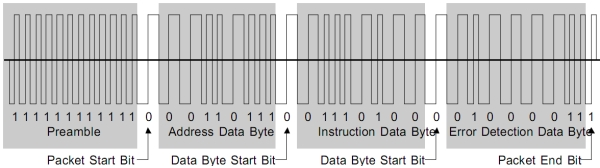
\includegraphics[scale=0.75]{trame.png}
\caption{Exemple d'une trame DCC}
\label{fig1}
\end{figure}

Ce protocole est un protocole standardis\'e qui permet de communiquer
entre la carte~\emph{FPGA} et les diff\'erents trains et
équipements de voies.
Il utilise une suite de commandes envoy\'ees sur les rails
jusqu'aux diff\'erents trains et composants qui agissent en fonction de
la commande qu'ils reçoivent.
La locomotive peut recevoir \'enormément de commandes différentes,
klaxon, annonces d'entr\'ee de gare, phares...(voir datasheet
locomotive). Elles ne seront pas toutes implement\'ees ici, mais
pourront \^etre rajout\'ees ult\'erieurement. 


\subsection{\underline{Le système d'enclenchement}}
\label{sec:logixl}

Le chapitre 2 du document \cite{sun2015} présente un système
ferroviaire. Un système ferroviaire est compos\'e de plusieurs systèmes~:
\begin{itemize}
  \item Les \'equipements de voie (rails, aiguillages...) et les
    trains. C'est la partie visible des passagers. 
  \item Le Poste de Commande ferroviaire qui permet à un \emph{op\'erateur} de
    visualiser, en temps r\'eel, l'\'etat du système (position des trains,
    position des aiguilles...)
  \item Le système d'enclenchement qui assure la s\'ecurit\'e du système
    ferroviaire. Il est plac\'e entre le Poste de Commande ferroviaire
    et les \'equipements de voie. Il interdit les commandes lorsque les
    conditions sont incompatibles avec la s\'ecurit\'e. 
\end{itemize}

La figure suivante pr\'esente les relations entre les diff\'erents
systèmes.\emph{(voir fig~\ref{fig3})}

\begin{figure}[h]
\centering
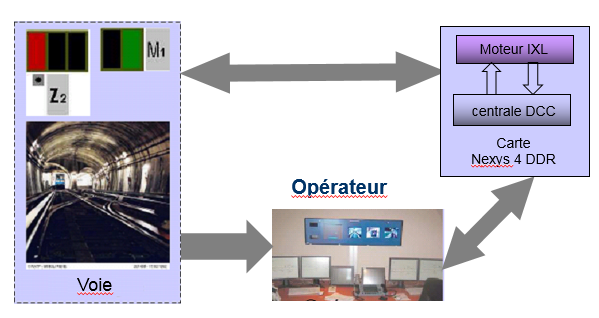
\includegraphics[scale=0.50]{sys_ferro.png}
\caption{Relation entre les différents systèmes}
\label{fig3}
\end{figure}

Un système d'enclenchement est initialement un système réalisé à base
d'un système de clenches (voir figure \ref{clenche}), puis de relais
mécanique (voir figure \ref{relais}). Lorsque les systèmes
d'enclenchement se sont 
informatisés, les relais ont été remplacés par des équations
booléennes (\cite{nyct2016}). Les équations booléennes sont basées sur
les mêmes principes que les relais.

\begin{figure}[ht]
    \begin{minipage}[c]{.46\linewidth}
        \centering
        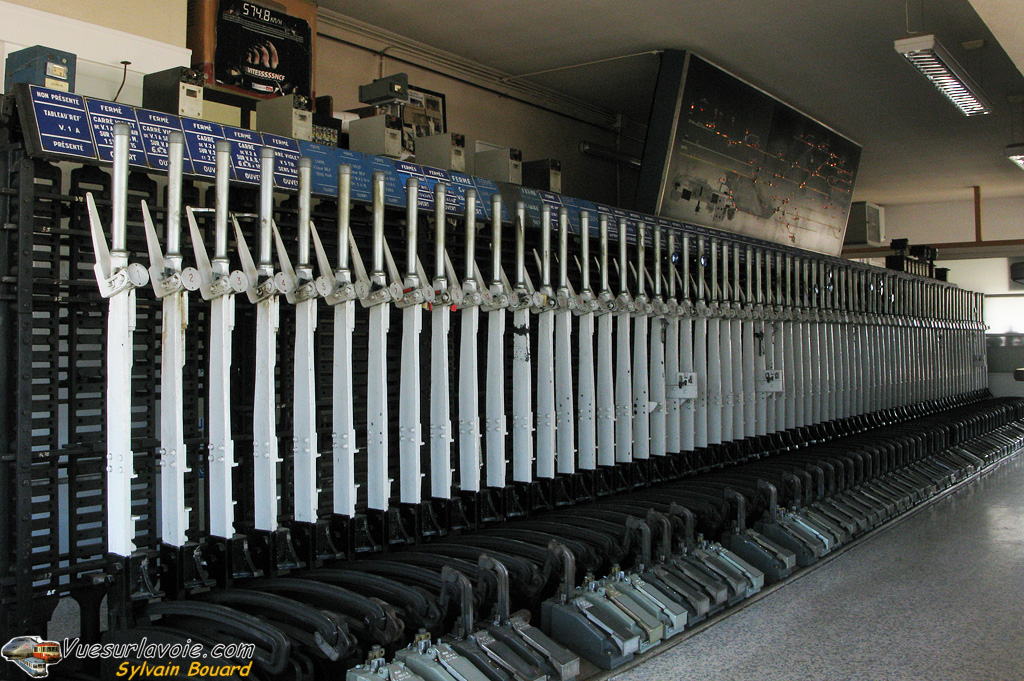
\includegraphics[scale=0.3]{enclenchement_mecanique.jpg}
        \caption{Enclenchement mécanique}
        \label{clenche}
    \end{minipage}
    \hfill%
    \begin{minipage}[c]{.46\linewidth}
        \centering
        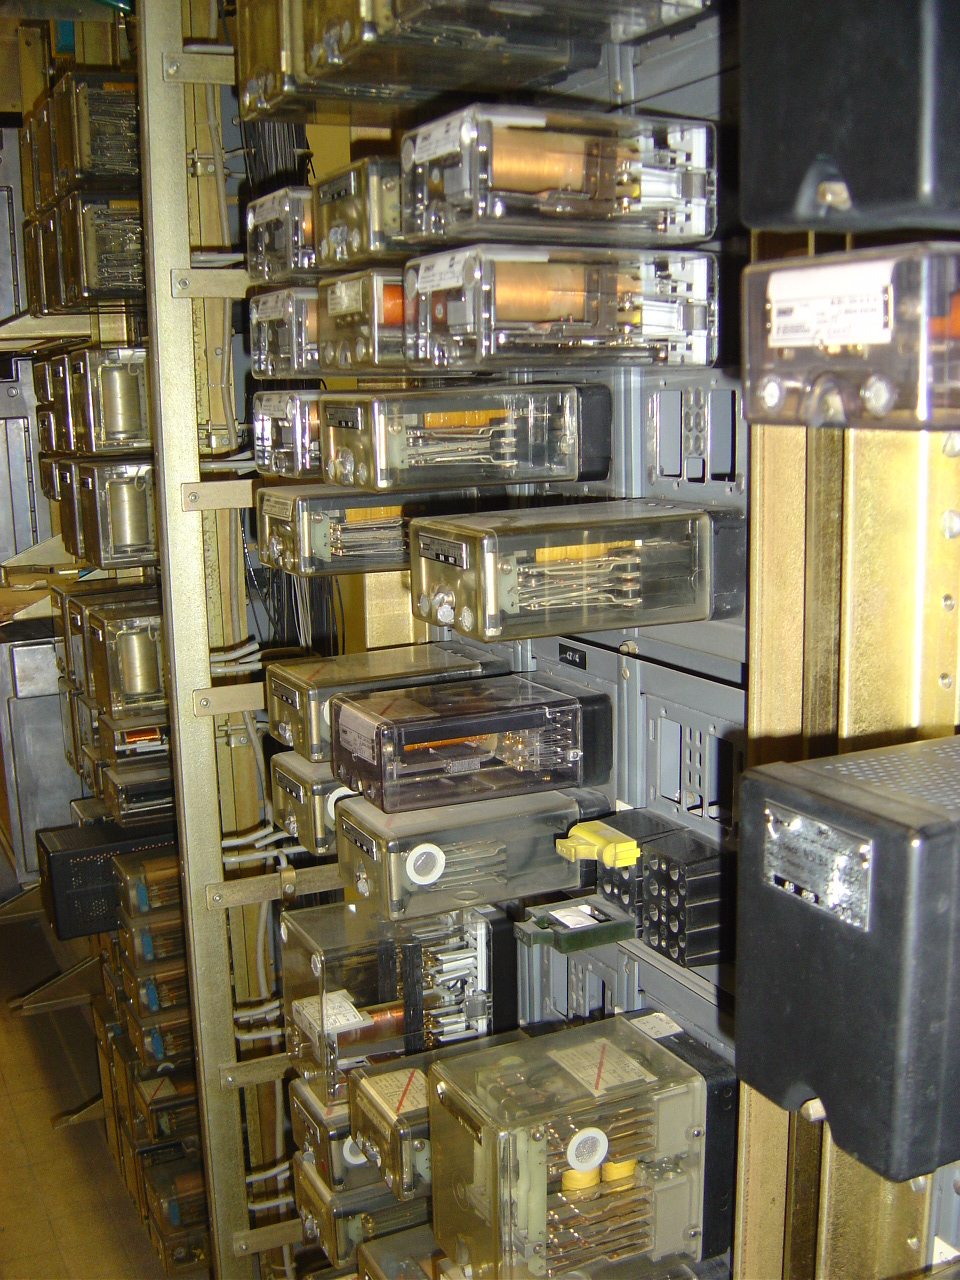
\includegraphics[scale=0.075]{enclenchement_relais.jpg}
        \caption{Enclenchement à relais}
        \label{relais}
    \end{minipage}
\end{figure}


La coeur de la gestion
  ferroviaire est la notion d'\emph{itinéraire} \cite{siteferro}. Un itinéraire
  représente la route entre 2 signaux\emph{(feu)}. Il contient les mouvements
  d'aiguilles nécessaires pour que le train parcourt le chemin entre le
  signal de départ et le signal d'arrivée. Le circuit ferroviaire ne
  contient pas de signaux, ils seront remplacés par des commandes de
  train. Un itinéraire peut être dans les états suivants:
  \begin{itemize}
  \item \emph{commandé}: L'opérateur demande au train de parcourir
      l'itinéraire choisi. Il a par conséquent demandé la formation de
      l'itinéraire au système d'enclenchement. Si les conditions sur
      les aiguilles à manoeuvrer pour former l'itinéraire sont
      correctes, le système d'enclenchement passe à l'état de formation de
      l'itinéraire sinon il est rejeté.
  \item \emph{formé}: Les aiguilles sont positionnées dans la bonne
      direction. Il n'est plus possible de bouger les aiguilles tant
      que le train se situe dans une certaine zone.
  \item \emph{détruit}: Le train a parcouru l'itinéraire, celui-ci peut
      être détruit de façon à autoriser le parcours d'un autre train sur les
      aiguilles.  
  \end{itemize}

\medskip
Un système d'enclenchement est composé d'enclenchements correspondant
chacun à une condition à vérifier. Par exemple, l'{enclenchement
d'approche d'une aiguille}; Il interdit la formation d'un 
nouvel itinéraire si un train se situe dans la "zone d'approche".
En effet, dans cette zone, un train
n'aurait pas la distance suffisante pour s'arrêter normalement devant
l'aiguille.  Sans cet enclenchement, l'opérateur pourrait détruire
l'itinéraire et commander un autre itinéraire. Le train, ne pouvant
s'arrêter correctement, arriverait sur une aiguille encore en
mouvement et déraillerait.
Sur la figure \ref{encl_approche}, lorsque le train se situe dans la
zone verte, il est possible de bouger l'aiguille A4. Si le train se
trouve dans le zone rouge, alors l'aiguille A4 est \emph{enclenchée}
et toute demande de mouvement de l'aiguille sera rejetée.

%\begin{figure}[h!]
%\centering
%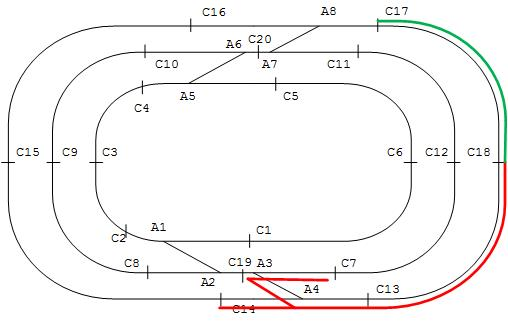
\includegraphics[scale=0.7]{zone_approche.jpg}
%\caption{Enclenchement d'approche d'aiguille}
%\label{encl_approche}
%\end{figure}

\begin{center}
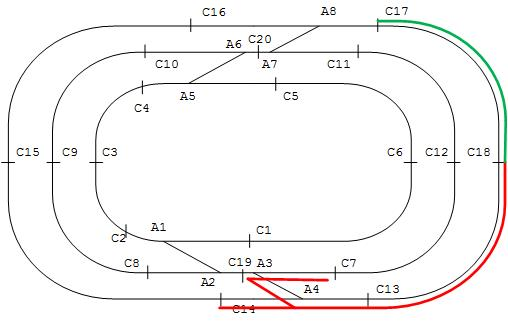
\includegraphics[scale=0.6]{zone_approche.jpg}
\captionof{figure}{Enclenchement d'approche d'aiguille}
\label{encl_approche}%
\end{center}

\newpage
  
La figure~\ref{archi} présente l'architecture retenue pour le
projet. Elle est composée de 3 parties~:
  \begin{itemize}
    \item La centrale DCC. Elle gère les Entrées/Sorties avec les
      équipements de voie et avec l'IHM. Elle fournit, à la logique
      d'enclenchement, l'état des commandes IHM et des équipements de
      voie et commande les trains. Ceci permet de séparer complètement
      la logique d'enclenchement, de la gestion informatique des
      Entrées/Sorties.
    \item La logique d'enclenchement. Elle contient les équations
      booléennes au format VHDL. 
    \item Le moteur d'instanciation. Il permet de générer, hors temps réel,
      la logique d'enclenchement au format VHDL à partir des équations
      booléennes.
  \end{itemize}

\begin{figure}[ht]
\centering
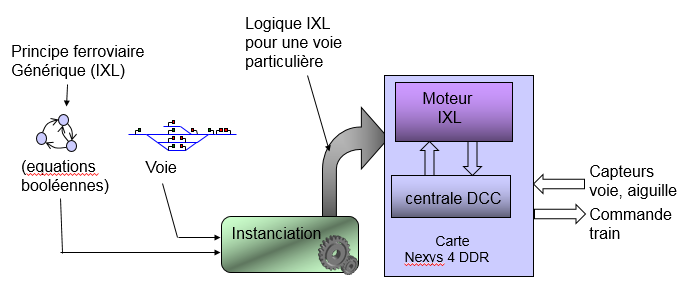
\includegraphics[scale=0.45]{moteur.png}
\caption{Architecture du projet}
\label{archi}
\end{figure}

Le moteur DCC a été développé en VHDL. Le moteur d'instanciation a été
développé en OCaml \cite{OCAML}.


\newpage
\subsection{\underline{Architecture g\'en\'erale du circuit de train}}
\label{sec:archi}

Voici le sch\'ema repr\'esentant l'installation ferroviaire utilis\'ee
tout au long du projet en mode simulation.

\begin{figure}[h]
\centering
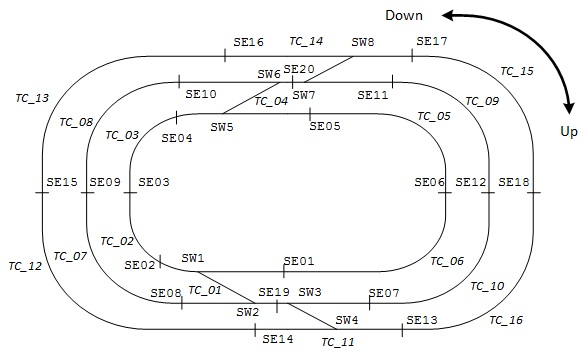
\includegraphics[scale=0.55]{circuit_complet.jpg}
\caption{Sch\'ema de l'installation}
\label{fig4}
\end{figure}

L'installation à partir de laquelle le projet a été développé est
 \emph{(voir fig~\ref{fig4})}, compos\'ee de 3
circuits imbriqués, de 4 paires d'aiguillages control\'ees par 8
contr\^oleurs gérés par trame DCC, et de 20 capteurs.
Le dispositif peut accueillir jusqu'\`a 6 trains en m\^eme temps.

\begin{figure}[h]
\centering
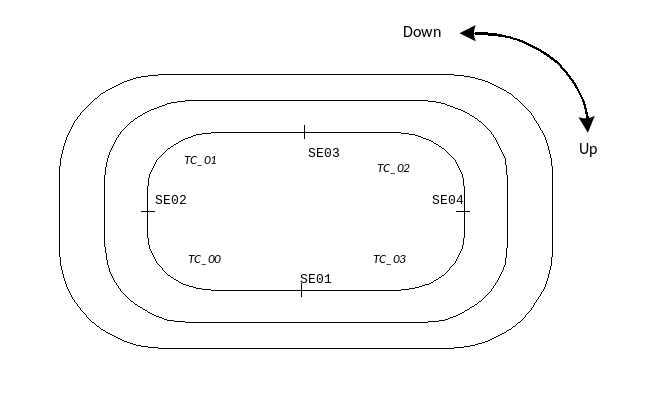
\includegraphics[scale=0.55]{circuit_vrai.png}
\caption{Sch\'ema de l'installation}
\label{schéma réél}
\end{figure}

Voici l'installation initiale dont je disposais lors de ce projet. Il n'y a pas
d'aiguillage et seulement 4 capteurs, donc incomplet pour les tests prévus.


\begin{figure}[h]
\centering
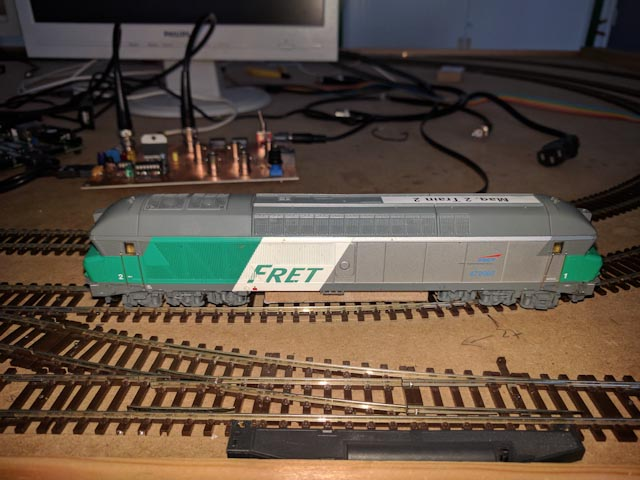
\includegraphics[scale=0.27]{loco.jpg}
\caption{Photo d'une locomotive}
\label{fig5}
\end{figure}

\newpage

Chaque locomotive poss\`ede une adresse sous forme de \emph{code
barre} sous elle \emph{(voir fig~\ref{fig6})}.

Le code barre est compos\'e de la façon suivante :
\begin{itemize}
    \item \textbf{un pr\'eambule} compos\'e de 2 bandes noires
      s\'epar\'ees par 1 bande blanche.
    \item \textbf{de l'adresse} le nombre de bandes noires correspond
      à l'adresse du train. 
    \item \textbf{un \'epilogue} compos\'e de 3 bandes noires
      s\'epar\'ees par 2 bandes blanches.
\end{itemize}

\begin{figure}[h]
\centering
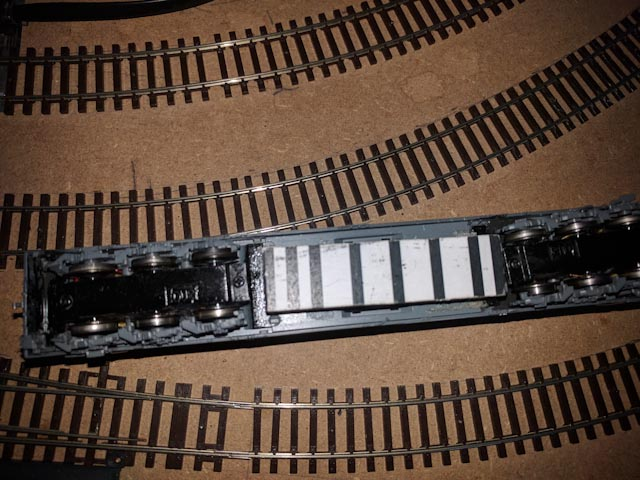
\includegraphics[scale=0.27]{add.jpg}
\caption{Photo de l'adresse sous la locomotive}
\label{fig6}
\end{figure}

Grâce aux capteurs une table contenant la
dernière position connue de chaque train peut être mise à jour ce qui va nous permettre de
choisir si un train doit changer de voie ou rester sur la sienne selon
si il y a un train qui bloque ou non la zone d'aiguillage qui nous concerne.


\subsection{\underline{Outils}}
\label{sec:outils}

Lors de ce projet, les diff\'erents outils suivants ont été utilisés:
\medskip
\begin{itemize}
  \item La carte \crt comme plateforme de d\'eveloppement
  \item La locomotive \emph{Jouef ``Fret SNCF``}\cite{Jouef}, les capteurs de
    position et des aiguillages
  \item Le protocole DCC \cite{DCC}
  \item Le logiciel Vivado comme \emph{IDE}
\end{itemize}
\medskip
ainsi que plusieurs langages:
\begin{itemize}
  \item \emph{VHDL}\cite{VHDL} comme language de description pour mes diff\'erentes
    \emph{IP}
  \item \emph{GIT}\cite{GIT} pour la gestion de configuration des logiciels
  \item \emph{\LaTeX}\cite{LATEX} pour la r\'edaction de la documentation
  \item Le langage \emph{Ocaml}\cite{OCAML} pour la g\'en\'eration de la logique d'enclenchement
\end{itemize}

\newpage
\section{Organisation du projet}
\label{sec:org_proj}

\subsection{\underline{Activit\'es du projet}}
\label{sec:activ}

Comme dit précédemment \emph{(voir \ref{sec:logixl})} le projet a \'et\'e
découp\'e en plusieurs \'etapes diff\'erentes, mais toutes n'ont pas été
possible à réaliser concrêtement car la maquette n'\'etait pas en \'etat de
fonctionnement complet.


Voici ce qui a \'et\'e r\'ealis\'e lors de ce projet.

\begin{enumerate}[1]
  \item Portage de la centrale DCC (fait)
  \begin{itemize}
    \item Création d'une nouvelle Interface
      Homme Machine
    \item Portage du code de l'ancienne centrale DCC et de la
      gestion des capteurs
  \end{itemize}

  \item Gestion des circuits de voie (réalisé uniquement en simulation)
  \begin{itemize}
    \item D\'efinition d'une interface entre le moteur DCC et le moteur IXL pour
      permettre la communication entre les 2 modules
    \item Cr\'eation d'un langage de d\'efinition pour la gestion des circuits
      de voie
    \item D\'efinition des \'equations g\'en\'eriques de gestion des circuits
      de voie
    \item Cr\'eation d'un langage pour la g\'en\'eration des sc\'enarios de
      simulation
    \item \'Ecriture des diff\'erents sc\'enarios de mouvement des trains.
  \end{itemize}

  
  \item Gestion des aiguillages (réalisé uniquement en simulation). Sur la
  base de la gestion des circuits de voie  
    \begin{itemize} 
      \item D\'efinition des \'equations g\'en\'eriques de gestion des aiguillages.
    \item \'Ecriture des diff\'erents sc\'enarios de mouvements des aiguillages.
    \end{itemize}
\end{enumerate}

La documentation associ\'e aux langages d'\'ecriture des \'equations
d'enclenchement et d'\'ecriture des sc\'enarios de simulation est
\'egalement fournie pour permettre de poursuivre le projet.


\newpage

\subsection{\underline{Planning pr\'evisionnel}}
\label{sec:planning}

Voici les différentes t\^aches ainsi que le planning initial qui devait être
respecté pour r\'eussir \`a mener \`a bien mon projet. La
figure~\ref{gantt} pr\'esente le diagramme de Gantt du projet. Ce planning m'a permis de vérifier l'avancement de mon projet au fur et à mesure.

\begin{figure}[h]
\centering
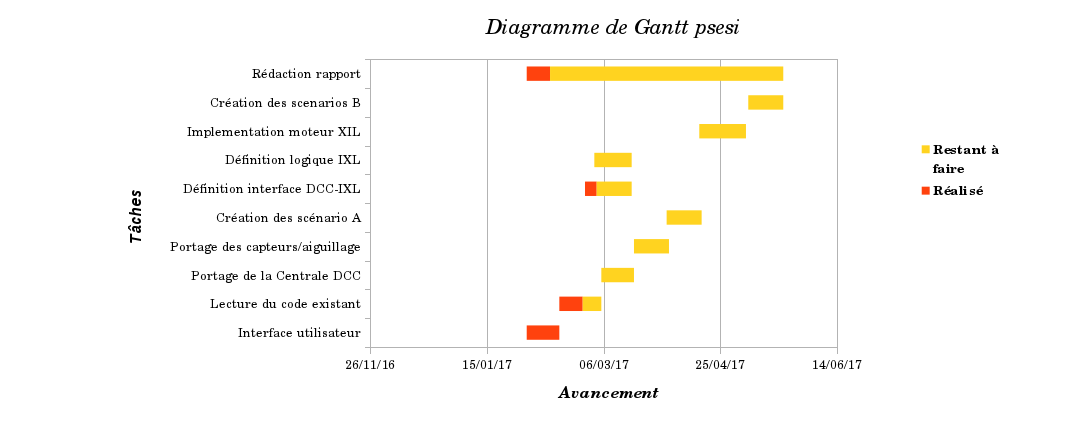
\includegraphics[scale=0.5]{gantt.png}
\caption{Diagramme de Gantt}
\label{gantt}
\end{figure}

\subsection{\underline{Gestion du projet}}
\label{sec:gestion}

Le projet a \'et\'e enti\`erement r\'ealis\'e en gestion de configuration avec l'outil \emph{GIT} (\cite{GIT}). L'annexe A pr\'esente l'arborescence de d\'eveloppement du projet.

Chaque morceau du projet peut \^etre compil\'e de fa\c con autonome et
automatique avec la commande \emph{make}.

La documentation a \'et\'e \'ecrite avec l'outil \LaTeX.

Les outils de g\'en\'eration de VHDL ont \'et\'e \'ecrit en \emph{OCaml}. Ce
langage permet un d\'eveloppement rapide de programme de manipulation de
structures complexes.


\subsection{\underline{Réalisation}}
\label{sec:Réal}

\subsubsection{\underline{Centrale DCC}}
\label{sec:Centrale}

La centrale DCC a été créée afin de pouvoir contrôler les
différents trains et équipements de voie dont nous pouvions
disposer (en simulation ou en réél).
\medskip
La centrale se base sur celle qui a été réalisée lors du cours de FPGA  \emph{(voir \cite{rapport} et \cite{sujet})}

La centrale est capable d'envoyer différentes \emph{trames DCC}
pour contrôler plusieurs équipements à la fois. Voici les différentes
commandes que l'on peut gérer avec l'interface.


\begin{itemize}
    \item le choix de \textbf{l'adresse} du \emph{train} qui va
      recevoir la commande
    \item le choix de la \textbf{vitesse} que \emph{le train} s\'electionn\'e
      va recevoir. 
    \item le choix  \textbf{du numéro} de la \emph{route} \`a \'etablir.
    \item les \textbf{features} qui pourront \^etre rajout\'ees au
      projet. 
  \end{itemize}


\begin{figure}[h]
    \begin{minipage}[c]{.46\linewidth}
        \centering
        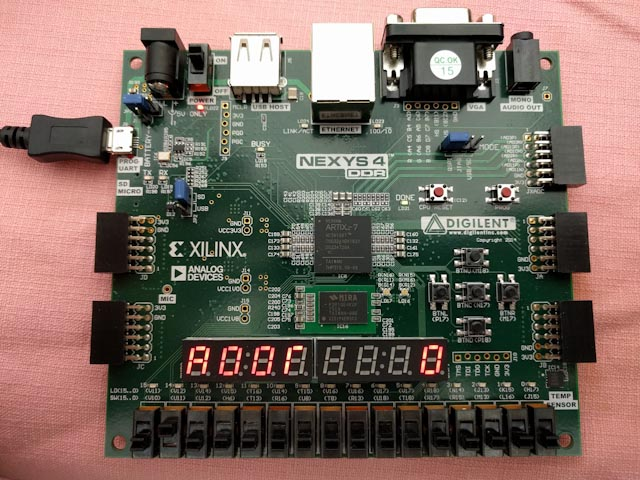
\includegraphics[scale=0.3]{exe_add.jpg}
        \caption{Exemple d'utilisation de la carte}
        \label{carte1}
    \end{minipage}
    \hfill%
    \begin{minipage}[c]{.46\linewidth}
        \centering
        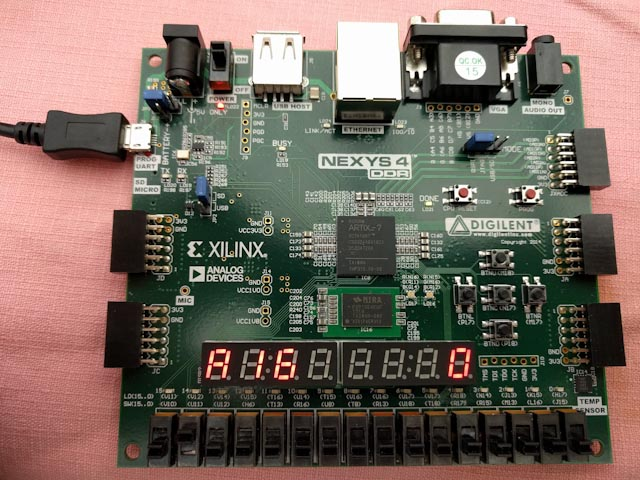
\includegraphics[scale=0.3]{exe_aigui.jpg}
        \caption{Exemple d'utilisation de la carte}
        \label{carte2}
    \end{minipage}
\end{figure}

La \emph{figure~\ref{carte1}} et la \emph{figure~\ref{carte2}} sont un
exemple du rendu de l'IHM d\'evelopp\'ee.
La \emph{figure~\ref{carte1}} représente la valeur de l'adresse du
train à qui on envoie la commande.
Tandis que la \emph{figure~\ref{carte2}} montre le numéro de
l'aiguillage que l'on veut bouger.
En appuyant sur le bouton gauche on change le réglage, et en appuyant sur le
bouton droit on incrémente la valeur du réglage choisi.
Le premier switch de la carte sert à réinitialiser les différentes
valeurs de la centrale \emph{(adresse, commande..)}.

\newpage

\subsubsection{\underline{Générateur moteur}}
\label{sec:Générateur}


Afin de pouvoir avoir un moteur d'interlocking modulable et adaptable
à différents types de circuits, j'ai utilisé un générateur de vhdl en
Ocaml qui prend en entrée un fichier contenant  différentes
équations selon l'exemple vi-dessous.

\emph{T\_16 <= ~SE\_UP\_18 * ~SE\_DO\_13 * (TC\_16 + SE\_DO\_18 + SE\_UP\_13);}


Le format des équations est le suivant :


On commence par le nom de la variable (T\_16), les variables utilisables sont
indiquées dans le fichier lexer\_simul.mll du répertoire Simul, suivi
d'un ``<='' 

Ensuite on met l'équation logique qui nous intéresse suivant la syntaxe suivante:
syntaxe :
\begin{enumerate}[->]
    \item \emph{\~} pour le \textbf{not}
    \item \emph{+} pour le \textbf{ou}
    \item \emph{*} pour le \textbf{et}
    \end{enumerate}

\medskip

Les équations mal écrites nous retourne une erreur et le fichier vhdl
ne sera pas généré.

\newpage

Le générateur est découpé en 5 fichiers
\begin{itemize}
   \item main.ml
   \item logic.ml
   \item ixl\_t.ml
   \item utils\_y.ml
   \item lexer\_simul.mll
\end{itemize}  

\medskip

Pour générer l'exécutable de l'application l'instruction suivante doit être lancée:

\begin{lstlisting}

   make clean depend all

\end{lstlisting}
  
\medskip

Le principe général de l'application est de parser le fichier.eq pour
en extraire les différentes équations qui seront ensuite transformées en
équations lisibles en vhdl.

\medskip

Il y a déja l'entête et l'épilogue du fichier écrit dans ``ff`` qui
permet à l'utilisateur de ne pas s'occuper de l'interface et de se
concentrer sur les équations voulues.

\medskip

Pour lancer l'application qui va créer le moteur IXL correspondant à la logique décrite il faut taper l'instruction suivante:

\begin{lstlisting}

   ./tanslate -i fichier.eq -o fichier\_out.vhdl

\end{lstlisting}




Le fichier en entrée est un fichier.eq qui reprend la syntaxe des
équations logiques dont la définition a été indiquée précédemment  \cite{}.
Et le fichier de sortie sera le moteur IXL généré contenant les
différentes équations du fichier d'entrée.

\newpage

\subsubsection{\underline{moteur IXL}}
\label{sec:IXL}

Voici l'interface du moteur IXL que nous allons utiliser :

\begin{lstlisting}[language=vhdl]
entity Ixl is  

  Port (
         -- synchro   
         CLK        : in  STD_LOGIC;
         reset      : in  STD_LOGIC;

         -- input
         valid_in   : in  STD_LOGIC; 
         Sw_Cmd_Req : in  STD_LOGIC_VECTOR (7 downto 0);
         Sw_State   : in  STD_LOGIC_VECTOR (7 downto 0);
         Sensor     : in  SE_state;
         
         -- output
         valid_out  : out STD_LOGIC;
         Sw_Cmd_Aut : out Sw_cmd_aut_t;

         --debug output
         TC_out     : out TC_St
         );

end Ixl;

\end{lstlisting}

Pour la sychronisation nous avons deux signaux, la clock et le signal
de reset \emph{actif haut}.

Il y a 4 signaux d'entrée :

\begin{itemize}
  \item valid\_in qui indique si on doit prendre en compte ou non les
    autres signaux.
  \item Sw\_Cmd\_Req qui contient l'état des aiguillages que l'on veut obtenir
  \item Sw\_State qui contient l'état actuel des aiguillages.
  \item Sensor qui contient les informations des différents capteurs à
    un instant donné.
\end{itemize}  

\medskip

Et 2 signaux de sortie :

\begin{itemize}
  \item valid\_out qui indique si l'on doit tenir compte des autres
    valeurs de sorties ou non.
  \item Sw\_Cmd\_Aut qui contient l'état des aiguillages que l'on demande.
\end{itemize}  

\medskip

Pour les simulations j'ai rajouté en sortie \emph{TC\_Out} qui permet
d'afficher l'état des \emph{Track Circuit} pour pouvoir suivre les
différents trains en cours de déplacement.

Pour voir la définition des différents types et leurs valeurs \emph{voir \cite{interface}}.

\bigskip

\textbf{Le fonctionnement}

Nous ne faisons la suite uniquement que si le signal \emph{valid\_in} est égal à '1'.

Nous mettons à jour toutes les nouvelles valeurs des \emph{Track
  Circuit} grâce au équations générées.

Puis nous mettons à jour les valeurs de sortie des différents
aiguillages selon les valeurs des Tracks Circuits.

\smallskip

Voir \cite{interface} pour avoir les différentes équations pour chaque Track
Circuits et pour les aiguillages.

\subsubsection{\underline{Test Bench}}
\label{sec:Test_Bench}

Voici les différents scénarios que j'ai utilisé comme base de test,
d'autres scénarios peuvent être créés  grâce au générateur de test.

\medskip

\begin{itemize}
    \item 1 train doit passer de la voie ``A`` à la voie ``B``
    \item 2 trains sur la voie ``A``, un seul doit passer sur la voie ``B``
    \item 1 train 1 sur voie ``A`` qui s'arrête dans la zone aiguillage.
          1 train 2 sur voie ``B``qui veut passer en voie ``A`` --> Pas
          possible. Red\'emarrage train 1, v\'erification du
          changement  de voie du train 2.
\end{itemize}

\medskip

Afin de pouvoir créer des tests facilement et de pouvoir essayer une
grande quantité de scénarios j'ai mis en place un générateur de test
qui reprend le principe du générateur du moteur IXL.

\smallskip

Le générateur se créé de la même façon que l'autre :

\begin{lstlisting}

   make clean depend all

\end{lstlisting}
  
\medskip

Pour générer le fichier vhdl de simulation il faut lancer l'instruction suivante:

\begin{lstlisting}

   ./simul.x -i fichier.simu -o IXL_tb.vhdl 

\end{lstlisting}

\medskip

Le fichier de sortie doit absolument se nomer IXL\_tb.vhdl si l'on
veut pouvoir utiliser le makefile générant le fichier.vcd permettant
d'obtenir le chronogramme du test et d'avoir les résultats des
différents tests

\medskip

Voici la syntaxe des fichiers .simu pour un cycle donné.

\begin{lstlisting}

   Cycle 4 :
   Events
     SE_ID_2;  
     SE_UP_3;  -- enter into TC3	
   Outputs
     TC_02 = Free;
     TC_03 = Occ;  

\end{lstlisting}

\medskip

Il faut commencer par indiquer le numéro de cycle que l'on est entrain
d'écrire, cela servira pour le debug de l'application et l'affichage
des tests.

\medskip

Dans la partie \textbf{Events} il faut indiquer les signaux en entrée que nous
voulons voir changer. Toutes les variables que nous pouvons modifier
sont indiquées dans le fichier lexer\_simul.mll 

\medskip

Ensuite dans la partie \textbf{Outputs}, il faut indiquer les tests
que nous voulons réaliser.
Pour le générateur de test, si on veut que les test soient générés il
faut mettre des commentaires ``--''.

\bigskip

Pour chaque scénario ajouter les chronogrammes et tout...

\subsection{\underline{Conclusion}}
\label{sec:Conclusion}

Ce projet a été très compliqué à réaliser, mais vraiment très intéressant.Je me suis aperçu que la pré-étude était vraiment très importante car les questions que je me suis posées à ce moment-là m'ont permis d'anticiper un certain nombre de problèmes.


\newpage

\bibliographystyle{plain}
\bibliography{biblio}

\end{document}
